% Created 2024-09-28 Sat 17:01
% Intended LaTeX compiler: pdflatex
\documentclass[11pt]{article}
\usepackage[utf8]{inputenc}
\usepackage[T1]{fontenc}
\usepackage{graphicx}
\usepackage{longtable}
\usepackage{wrapfig}
\usepackage{rotating}
\usepackage[normalem]{ulem}
\usepackage{amsmath}
\usepackage{amssymb}
\usepackage{capt-of}
\usepackage{hyperref}
\author{Blaine Mooers}
\date{\today}
\title{}
\hypersetup{
 pdfauthor={Blaine Mooers},
 pdftitle={},
 pdfkeywords={},
 pdfsubject={},
 pdfcreator={Emacs 29.4 (Org mode 9.6.15)}, 
 pdflang={English}}
\begin{document}

\tableofcontents

\chapter{Introduction}
\epigraph{In God we trust. All others must bring data.}{W. Edwards Deming}

\section{Introduction}
This is the introduction to Chapter 1.
Here you can provide an overview of the chapter's content.

\section{section 2}
\subsection{section 2.1}
This is the first subsection of Section 2.


\begin{figure}
    \centering
    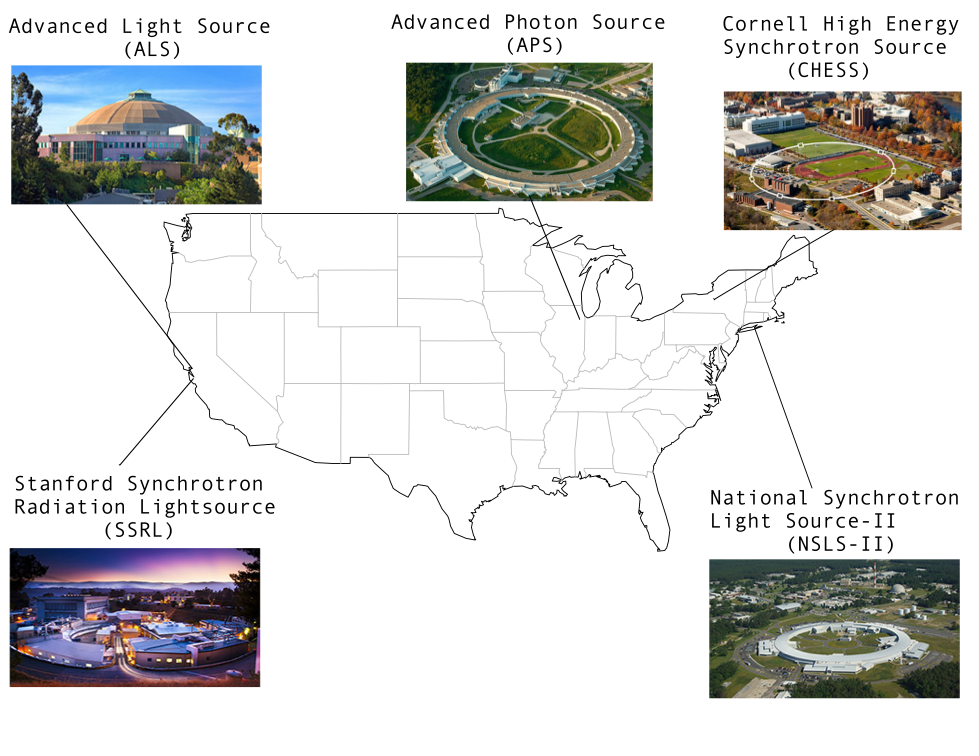
\includegraphics[scale=0.68]{./Contents/figs/LightSourcesUSA.png}
    \caption{This is the figure caption. \label{fig:LightSources}}
\end{figure}

\begin{table}[htbp]
\caption{This is the table caption.}
\centering
\begin{tabular}{rlllll}
Sample & Variable1 & Variable2 & Variable 3 & Variable 4 & \%ariable 5\\[0pt]
\hline
1 & q & u & o & p & y\\[0pt]
2 & q & u & o & p & y\\[0pt]
3 & q & u & o & p & y\\[0pt]
4 & q & u & o & p & y\\[0pt]
\end{tabular}
\end{table}


\begin{table}[h]
\begin{center}
\caption{This is a test.}
\begin{tabular}{ c c c }
\hline
A & B & C \\
\hline
 cell1 & cell2 & cell3 \\
 cell4 & cell5 & cell6 \\
 cell7 & cell8 & cell9
\hline
\end{tabular}
\end{center}
\end{table}

\subsection{Subsection 1.2}
This is the second subsection of Section 1.

\section{Section 2}
\subsection{Subsection 2.1}
This is the first subsection of Section 2.

\subsection{Subsection 2.2}
This is the second subsection of Section 2.

\section{Conclusion}
\index{index!Test}
This is the conclusion of Chapter 1. Summarize the key points discussed in the chapter.
\end{document}
